\documentclass{article}

% Packages for setting up page margins
\usepackage[margin=1in]{geometry}

\usepackage{graphicx, setspace, amsmath, mathtools, amssymb, url, float, listings}
\setlength{\parskip}{2mm}
\graphicspath{ {./images/} }

% Title
\title{CS535 Design and Analysis of Algorithms - Assignment 4}
\author{Batkhishig Dulamsurankhor - A20543498}
\date{\today} % Use \date{} for no date

\begin{document}

\maketitle

\begin{enumerate}
  \item To find the contradiction, we need to find all pairs of patients $(i,j)$ with $(h_i>h_j)$ and $(w_i<w_j)$ or $(h_i<h_j)$ and $(w_i>w_j)$.
  A trivial approach would be comparing each of patient's weight and height with every other's.
  This algorithm works but not efficient and takes $O(n^2)$.
  
  Instead, we can solve the problem with the following algorithm:
  \begin{itemize}
    \item Sort the patients by their heights in ascending order using algorithms like merge sort. This step takes $O(nlogn)$.
    \item Now we have list of patients ordered by their heights.
    If there is no contradiction here, weights should also be in ascending order.
    Merge sort has a really convenient pattern here to detect any contradiction in the hypothesis.
    When merging, everytime there when there is a $w_i>w_j$ where $h_i<h_j$, it chooses $w_j$ first and then $w_i$, ensuring the correct order.
    We can take advantage of this logic to count every contradiction pair.
    In short, we can sort the list again by their weights using merge sort and instead of just merging, we count the number of times when have to choose from the right list first before left list is empty.
    After this sort, we are left with the result.
    This step also takes $O(nlogn)$.
  \end{itemize}

  In total, the time complexity is $O(nlogn+nlogn)=O(nlogn)$.

  Algorithm pseudocode:

  \begin{lstlisting}

    merge(P, L, M, R):
      result=0
      i=L,j=M
      replacement=[]
      while i<M && j<R:
        if P[i].weight<=P[j].weight:
          replacement.add(P[i])
          i++
        else:
          result+=M-i+1
          replacement.add(P[j])
          j++
      P[L,R+1]=replacement
      return result

    merge_sort(P, L, R):
      result=0
      if (L<R):
        result+=merge_sort(P,L,(L+R)/2)
        result+=merge_sort(P,(L+R)/2+1,R)
        result+=merge(P,L,(L+R)/2,R)

    main(P):
      sort(P) by height;
      result=merge_sort(P, 0, length(P)-1)
      return result;

  \end{lstlisting}
  \item The tree $T$ is a perfect binary tree since it is a complete binary tree with $n=2^d-1$ nodes.
  For a node to be a local minimum, all its neighbors' values are more than its value.
  Because we are given a binary tree, there are at most $3$ neighbors, a parent and two children.
  A root has $2$ children neighbors and a leaf node has $1$ parent neighbor.

  We can achieve $O(logn)$ complexity with the following approach:

  \begin{itemize}
    \item We start from the root of $T$.
    \item We check the value of each of its neighbors and compare them with the current node's value.
    \item Then we go to the smallest value node.
    \item If the current node is the smallest, we found a local minimum.
  \end{itemize}

  This algorithm is correct because we only go down the tree and never go back up.
  Going back up to a parent means $x_{parent}<x_{child}$.
  However, we are moving down the tree only when the parent's value is more than at least one of its children's value.
  We would never go down to the child if $x_{parent}<x_{child}$ was the case in the first place.

  This means in the worst case scenario, the length of the traversal is only the depth of the binary tree $d$.
  The time complexity of this algorithm is therefore $O(d)$ and we know that $n=2^d-1$ so $d=log(n+1)$.
  This makes the time complexity $O(log(n+1))=O(logn)$.

  Algorithm pseudocode:

  \begin{lstlisting}

    local_min(T):
      if (T is leaf node):
        return T
      if (T.val<T.left.val && T.val<T.right.val):
        return T
      
      if (T.left.val<T.val && T.left.val<T.right.val):
        return local_min(T.left)
      else:
        return local_min(T.right)
    
    main(T):
      return local_min(T)

  \end{lstlisting}
  \item When $k$ is chosen to be $\sqrt{n}$ then the number of partition becomes $n/(2\sqrt{n}+1)$.
  
  \begin{itemize}
    \item We are given that finding a median of each group is $O(1)$ time. So for all columns it's $O(n)$.
    \item Finding median of median recursively: $FIND(M,\dfrac{n}{2(2\sqrt{n}+1)})$. $T(\dfrac{n}{2(2\sqrt{n}+1)})$
    \item Use median of median to partition takes $O(n)$.
    \item The rank of $p$ is:
    \begin{center}
      $\dfrac{n}{2(2k+1)}(k+1)\leq rank(p) \leq n-\dfrac{n}{2(2k+1)}(k+1)$
    \end{center}

    The number of items in paritions A and B. (This is taken from lecture note).
    Recursive call of the function is limited by the upper limit:
    
    \begin{center}
      $T(n-\dfrac{n}{2(2\sqrt{n}+1)}\sqrt{n}+1)=T(n\dfrac{4\sqrt{n}+2-\sqrt{n}-1}{4\sqrt{n}+2})=T(n\dfrac{3\sqrt{n}+1}{4\sqrt{n}+2})$
    \end{center}

  \end{itemize}

  The recurrence is therefore:

  \begin{center}
    $T(n)=O(n)+T(\dfrac{n}{2(2\sqrt{n}+1)})+O(n)+T(n\dfrac{3\sqrt{n}+1}{4\sqrt{n}+2})$
  \end{center}

  For sufficiently large $n$, $T(\dfrac{n}{2(2\sqrt{n}+1)})\approx T(\sqrt{n})$ and $T(n\dfrac{3\sqrt{n}+1}{4\sqrt{n}+2})\approx T(\dfrac{3}{4}n)$.
  We can neglect $T(\sqrt{n})$ for large $n$ too.
  So, the recurrence becomes:

  \begin{center}
    $T(n)=O(n)+T(\sqrt{n})+O(n)+T(\dfrac{3}{4}n)$

    $=O(n)+T(\dfrac{3}{4}n)$
  \end{center}

  If we plug in master theorem, we get:

  $a=3, b=4, d=1 \Rightarrow log_ba=log_43<1$

  \begin{center}
    $T(n)=O(n^d)=O(n)$
  \end{center}
  
  \item In this problem, I am assuming the greedy problem works by choosing the shortest edge first.
  Then we choose the next smallest edge unless it intersects the chosen edges.
  We keep running this until we are left with all triangles.

  \begin{figure}[H]
    \centering
    \begin{minipage}{0.4\textwidth}
      \centering
      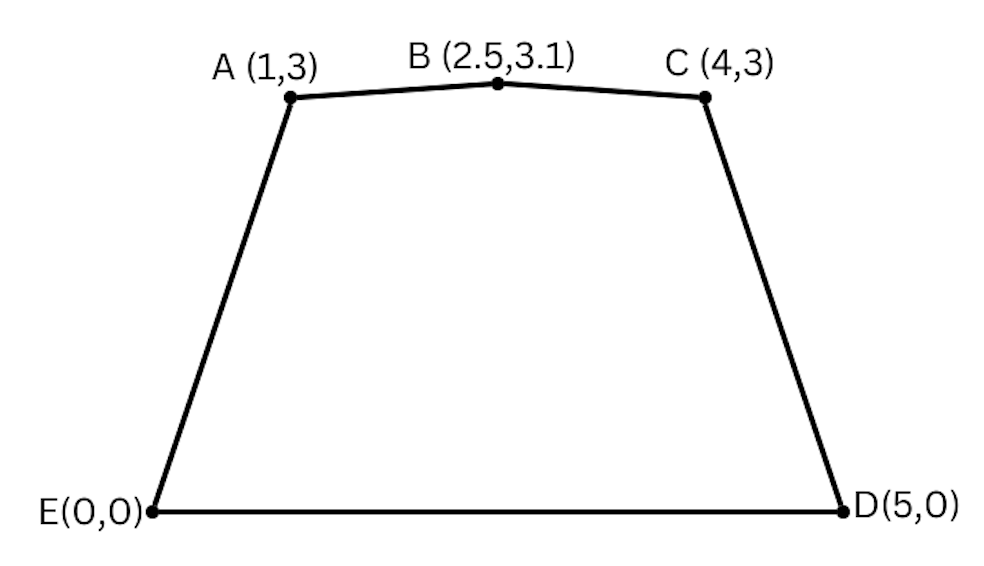
\includegraphics[width=\textwidth]{image1.png}
      \caption{We have the above 5 convex polygon points and we want to find non-intersecting diagonals that divides the pentagon to triangles.}
    \end{minipage}
    \hspace{1cm}
    \begin{minipage}{0.4\textwidth}
      \centering
      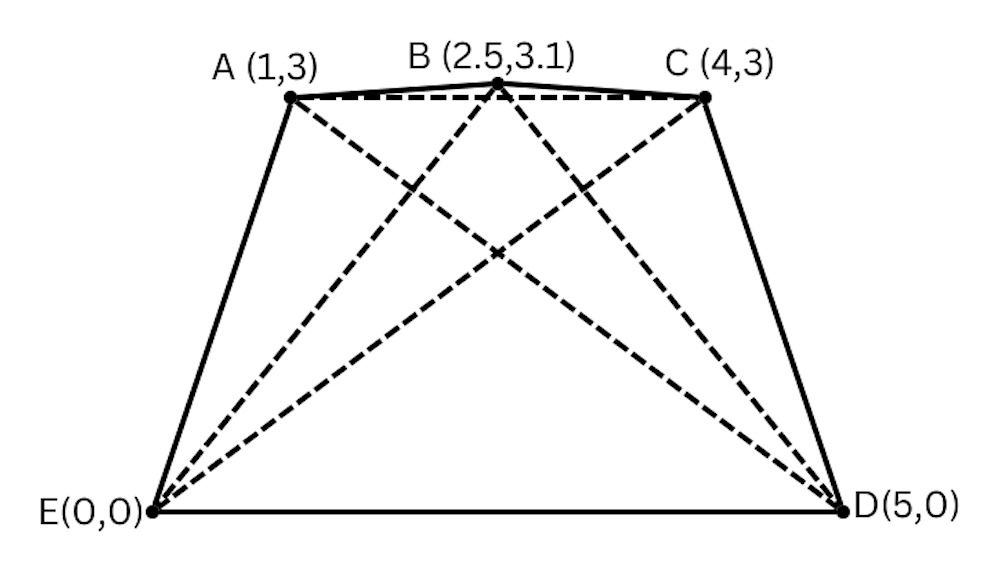
\includegraphics[width=\textwidth]{image2.png}
      \caption{There are total of 5 possible diagonals. We can choose $n-3=2$ of them to solve this problem.}
    \end{minipage}
  \end{figure}

  Let's calculate each of these diagonal's lengths.

  \begin{itemize}
    \item $l_{AC}=\sqrt{(4-1)^2+(3-3)^2}=\sqrt{9}=3$
    \item $l_{AD}=\sqrt{(5-1)^2+(0-3)^2}=\sqrt{25}=5$
    \item $l_{BD}=\sqrt{(5-2.5)^2+(0-3.1)^2}=\sqrt{25}=3.98$
    \item $l_{BE}=\sqrt{(0-2.5)^2+(0-3.1)^2}=\sqrt{25}=3.98$
    \item $l_{CE}=\sqrt{(0-4)^2+(0-3)^2}=\sqrt{25}=5$
  \end{itemize}

  The order of the length: $l_{AC}<l_{BD}=l_{BE}<l_{AD}=l_{CE}$

  \begin{figure}[H]
    \centering
    \begin{minipage}{0.4\textwidth}
      \centering
      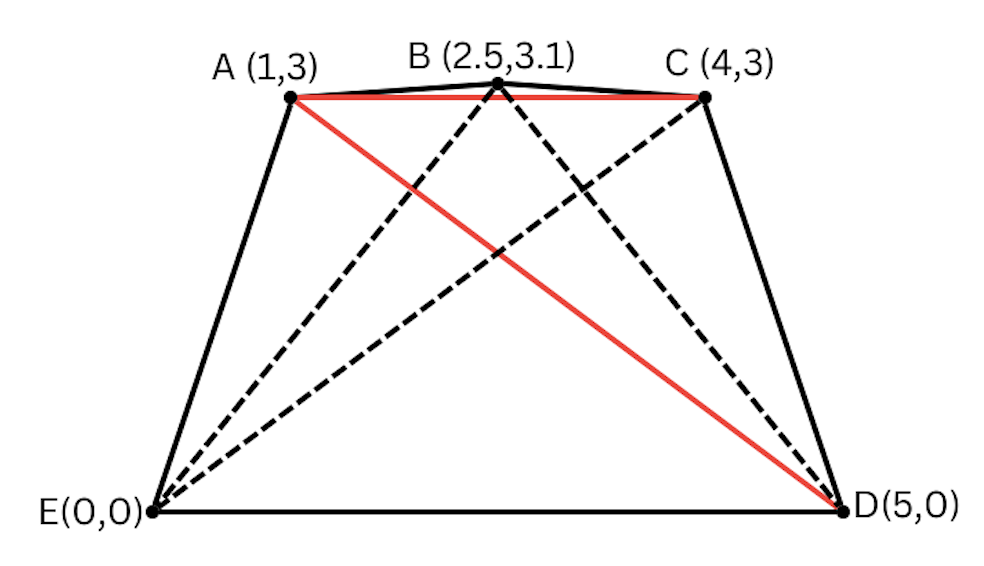
\includegraphics[width=\textwidth]{image3.png}
      \caption{If we run greedy algorithm, we choose AC diagonal first because it is the shortest.
      Then, we can choose either BD or BE, but since they both cross AC, we skip.
      So, we can either choose AD or CE and let's say we choose AD.
      The result is, AC and AD with total length $l_{AC}+l_{AD}=3+5=8$.}
    \end{minipage}
    \hspace{1cm}
    \begin{minipage}{0.4\textwidth}
      \centering
      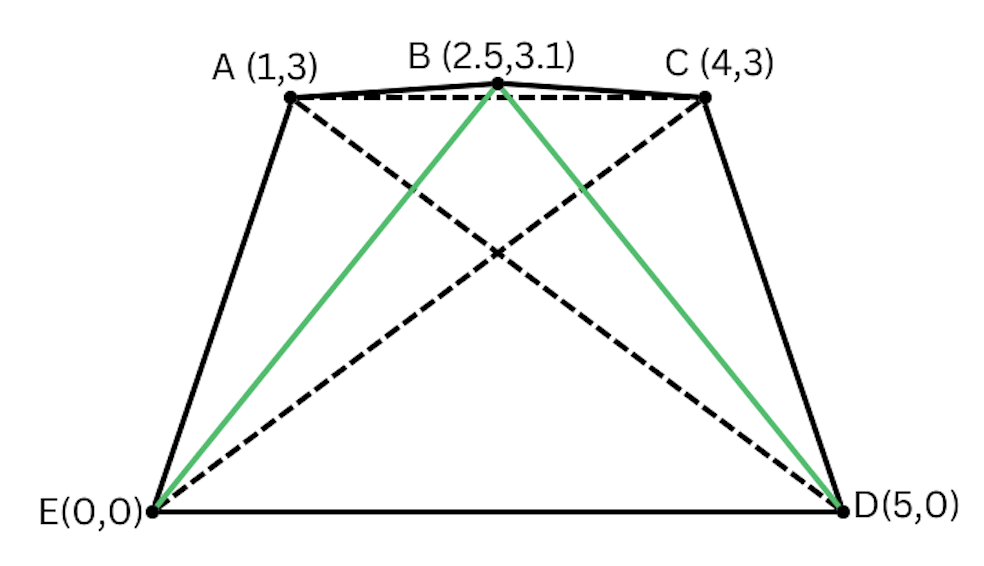
\includegraphics[width=\textwidth]{image4.png}
      \caption{However, the optimal solution is not AC and AD.
      We actually have a better solution, that doesn't contain the shortest diagonal in this polygon.
      If we choose BE and BD, the total length is $l_{BE}+l_{BD}=3.98+3.98=7.96$, which is less than 8.
      Therefore, dynamic programming will yield the optimal result and not necessarily greedy algorithm.}
    \end{minipage}
  \end{figure}

  \item Since we are given a single processor, we can't choose jobs that have overlapping range.
  We can't use greedy algorithm here because profit is associated with the jobs.
  So we can solve this using dynamic programming.
  The algorithm works as follows:
  \begin{itemize}
    \item We sort the jobs by their finish time.
    (Similar to how greedy algorithm works for job scheduling problem without profit)
    \item We initialize dp array with size of the number of jobs and solve the problem bottom to up.
    In the dp array, we save the maximum profit after finishing time for each job.
    We also initialize subsets array for keeping the current subset of jobs.
    \item To achieve this, we need to calculate whether including the current job can yield maximum profit or not.
    If it exceeds the maximum profit, we include it or else, we don't include it and keep the previous maximum profit.
    \item We can calculate the current maximum profit by searching the job that has max finish time and non-overlapping to the current job.
    By using binary search, we can efficiently find such a job.
    \item After running these jobs, we return the last value in the subsets array, which is the subset of maximum possible profit.
  \end{itemize}

  \begin{lstlisting}

    search(J, i):
      // implementation of binary search
      // that returns one of the previous jobs that has maximum finish time
      return idx

    sort(J) by finish time
    dp[size of J]
    dp[0] = J[0].profit

    subsets[size of J]
    subsets[0] = [J[0]]

    for (i=1; i<J.size; i++):
      idx = search(J, J[i])
      if (J[i].profit+dp[idx] > dp[i-1]):
        subset[i] = [subsets[idx] + [J[i]]]
        dp[i] = J[i].profit+dp[idx]
      else:
        subset[i] = subset[i-1]
        dp[i] = dp[i-1]
    
    return subsets[-1]
  \end{lstlisting}

  The time complexity:

  \begin{itemize}
    \item sorting jobs $O(nlogn)$.
    \item populating dp array for each job $O(nlogn)$ (n for each iteration, logn for binary search).
  \end{itemize}

  The total time complexity is $O(nlogn)$.

  \item We can solve this problem also with dynamic programming.
  The intuition is that for each day, we save the longest valid subsequence of days that ends with that date.
  
  Algorithm:

  \begin{itemize}
    \item Initialize dp array by the size $n$ number of days.
    In the dp array, we save the longest subsequence that ends with the corresponding date.
    \item For a day $i$, we obtain the maximum length dp value of previous days if the price is lower than the previous date.
    Then we update current date's dp value by the previous maximum dp sequence added by the current day price.
    This way, we can calculate the longest rising sequence of days that ends with the current day $i$.
    \item After running this algorithm, iterate over each subsequence of dp and return the longest subsequence.
  \end{itemize}

  \begin{lstlisting}
    dp[n]
    dp[0]=[V[0]]
    for (i=1;i<n;i++):
      for (j=0;j<i;j++):
        if (V[j]<V[i] && len(dp[i])<len(dp[j]+1)):
          dp[i]=dp[j]+[V[i]]
    
    result=[]
    max_len=0
    for (i=1;i<n;i++):
      if (len(dp[i])>max_len):
        result=dp[i]
        max_len=len(dp[i])
    
    return result
  \end{lstlisting}

  The time complexity:

  \begin{itemize}
    \item populating dp array for each day $O(n^2)$.
    \item finding the longest subsequence in dp array $O(n)$.
  \end{itemize}

  The total time complexity: $O(n^2+n)=O(n^2)$.

\end{enumerate}


\end{document}